\documentclass[a4paper,12pt]{report}
\usepackage[utf8]{inputenc}
\usepackage[czech]{babel}
\usepackage{amsmath}
\usepackage{geometry}
\usepackage{xcolor}
\usepackage{graphicx}
\usepackage{fancyhdr}
\usepackage{soul}
\usepackage{array}
\usepackage{pgf}
\usepackage{enumitem}
\usepackage[normalem]{ulem}
\usepackage{hyperref}

\geometry{top=2.5cm, bottom=2.5cm, left=2.0cm, right=2.0cm}

% Variables, fill it here!
\newcommand{\sourceId}   {166}
\newcommand{\studentName}{Bc. Pavel Mikula}
\newcommand{\studentID}  {MIK0486}
\newcommand{\teacherName}{Ing. Michal Béreš, Ph.D.}

\renewcommand{\headrulewidth}{0pt}
\renewcommand{\footrulewidth}{0pt}

% Table and Image references
\newcommand{\tabref}[1]{Tab. \ref{#1}}
\newcommand{\figref}[1]{Obr. \ref{#1}}

% TODO command, to show spaces where to fill requested values more easily
\newcommand{\TODO}{\mbox{\textbf{\textcolor{red}{...} }}}

\pagestyle{fancy}
\fancyhead[L]{\colorbox{yellow}{\parbox{\dimexpr\textwidth-2\fboxsep\relax}{Jméno: \studentName}}}
\fancyhead[C]{\colorbox{yellow}{\parbox{\dimexpr\textwidth-2\fboxsep\relax}{}}}
\fancyhead[R]{\colorbox{yellow}{}{Číslo zadání: \sourceId}}

% Type of table columns that orients text to center
\newcolumntype{P}[1]{>{\centering\arraybackslash}p{#1}}

\begin{document}
\thispagestyle{empty}
\setcounter{page}{0}

% Title and header section
\begin{center}
    
\includegraphics[width=0.8\textwidth]{assets/logo.png} \\[4em]
    \vspace{4em}
    \textbf{PRAVDĚPODOBNOST A STATISTIKA} \\
    \vspace{1em}
    \textbf{Domácí úkoly 1S \textendash\ 3S} \\
    \textbf{\colorbox{yellow}{Zadání \sourceId}} \\
\end{center}

% Student information, values are implemented in variable section above
\vspace{2em}
\hspace{3em}
\begin{tabular}{ll}
    \textbf{Jméno studentky/studenta:}  & \hspace{6em} \studentName \\[0.5em]
    \textbf{Osobní číslo:}              & \hspace{6em} \studentID   \\[0.5em]
    \textbf{Jméno cvičící/cvičícího:}   & \hspace{6em} \teacherName \\
\end{tabular}

% Table with results
\vspace{10em}
\begin{center}
    \renewcommand{\arraystretch}{1.3}
    \begin{tabular}{|p{8em}|P{10em}|P{10em}|}
        \hline
                        & \textbf{Datum odevzdání}  & \textbf{Hodnocení}    \\ \hline
        Domácí úkol 1:  & 17.11.2024                &                       \\ \hline
        Domácí úkol 2:  &                           &                       \\ \hline
        Domácí úkol 3:  &                           &                       \\ \hline
        Celkem:         & ------------------------  &                       \\ \hline
    \end{tabular}
\end{center}

% Footer section
\vspace{5em}
\begin{center}
    \textbf{Ostrava, AR 2024/2025}
\end{center}

%\newpage
%\section*{Popis datového souboru}
\label{sec:data-source-description}

V datovém souboru jsou zaznamenány výkonnostní skóre (FPS) čtyř populárních grafických karet:
Nvidia RTX 2080 Ti, Nvidia RTX 3070 Ti, AMD Radeon RX 6800 XT a AMD Radeon RX 7700 XT. Tyto karty
byly testovány ve hře "Cyberpunk 2077" ve dvou různých verzích: původní release a po aplikaci 1.5
patche. Vaším úkolem je analyzovat, jak patch 1.5 ovlivnil výkonnostní skóre těchto karet ve hře. Pro
každý unikátní testovaný systém (test) viz (id) byly testovány obě verze hry

\vspace{1em}
\noindent
V souboru ukol\_X.xlsx jsou pro každý test uvedeny následující údaje:

\begin{itemize}
  \item \textbf{id} ... identifikátor testovaného systému (každý systém je unikátní PC systém)
  \item \textbf{typ karty} ... Nvidia RTX 2080 Ti, Nvidia RTX 3070 Ti, AMD Radeon RX 6800 XT, AMD Radeon RX 7700 XT
  \item \textbf{testovaná verze} ... „release“ a „patched“
  \item \textbf{FPS} ... naměřené výkonnostní skóre (FPS) pro danou grafickou kartu s danou verzi hry.
\end{itemize}

\noindent
Obecné pokyny:

\begin{itemize}
    \item Domácí úkoly odevzdávejte vždy v termínu, který určil váš cvičící.
    \item Portfolio domácích úkolů budete odevzdávat postupně. Tj. nejdříve odevzdáte titulní stránku s úkolem 1, k okomentovanému úkolu 1 připojíte úkol 2 atd
    \item Domácí úkoly zpracujte dle obecně známých typografických pravidel. 
    \item Všechny tabulky i obrázky musí být opatřeny titulkem, který obsahuje i očíslování objektu.  
    \item Do domácích úkolů nevkládejte tabulky a obrázky, na něž se v doprovodném textu nebudete odkazovat.
    \item Bude-li to potřeba, citujte zdroje dle mezinárodně platné citační normy ČSN ISO 690.
\end{itemize}

\endinput

\newpage
\section*{Úkol 1}
\label{sec:task-1}

Pomocí nástrojů explorační analýzy zkoumejte nárůst výkonnostních skóre (FPS) po aplikaci 1.5 patche 
(tj. rozdíl výkonnostních skóre pro verzi „patched“ a verzi „release“) ve hře "Cyberpunk 2077" pro grafické karty 
\nvidiaCard\ a \amdCard\. Data vhodně graficky prezentujte (krabicový graf, histogram, q-q graf)
a doplňte následující tabulku a text.

\vspace{2em}
\noindent
Výsledky popisné statistiky lze vidět v \tabref{tab:characteristics-summary} a na  \figref{fig:box_plot}, \figref{fig:histogram} a \figref{fig:qq}.

% Fill your table values here :)
\newcommand{\rangeValues}       {70,        59,         69,         58}
\newcommand{\minValues}         {-4.8,      4.2,        5.1,        4.2}
\newcommand{\QfValues}          {5.425,     4.900,      5.500,      4.900}
\newcommand{\medianValues}      {5.700,     5.300,      5.700,      5.300}
\newcommand{\meanValues}        {5.600,     5.371,      5.750,      5.191}
\newcommand{\QtValues}          {6.100,     5.550,      6.100,      5.500}
\newcommand{\maxValues}         {6.6,       15.8,       6.6,        5.9}
\newcommand{\sdValues}          {1.335,     1.452,      0.439,      0.451}
\newcommand{\cvValues}          {23.8,      27.0,       7.6,        8.7}
\newcommand{\skewnessValues}    {-6.9,      6.4,        0.2,        -0.4}
\newcommand{\kurtosisValues}    {51.3,      43.8,       -1.0,       -0.7}
\newcommand{\lowerBoundValues}  {4.41,      3.92,       0,          0}
\newcommand{\upperBoundValues}  {7.11,      6.52,       0,          0}

% Additional values
\newcommand{\sigmaValues} {4.873, 6.628, 4.289, 6.093}

% Helper command to put everything in table.
\newcommand{\tableValue}[2]{%
    \pgfmathparse{{#1}[#2]}%
    \edef\tempResult{\pgfmathresult}%
    \ifnum\pdfstrcmp{\tempResult}{inf}=0 %
        $\infty$%
    \else%
        \mbox{\tempResult}%
    \fi%
}

% Fuckin graphic card names
\newcommand{\nvidiaCard}{Nvidia RTX 3070 Ti}
\newcommand{\amdCard} {AMD Radeon RX 7700 XT}

\begin{table}[h!]
    \caption{Nárůst výkonnostních skóre (FPS) po aplikaci 1.5 patche ve hře "Cyberpunk 2077" pro grafické karty \nvidiaCard\ a \amdCard\ (souhrnné statistiky)}
    \label{tab:characteristics-summary}
    \vspace{0.5em}
    \renewcommand{\arraystretch}{1.3}
    \resizebox{\textwidth}{!}{%
        \begin{tabular}{|p{3.5cm}|P{3cm}|P{3cm}|P{3cm}|P{3cm}|}
            \hline
                                  & \multicolumn{2}{P{6cm}|}{\textbf{Původní data}}                   & \multicolumn{2}{P{6cm}|}{\textbf{Data po odstranění odlehlých pozorování}} \\ \hline
                                  & \centering \textbf{\nvidiaCard} & \textbf{\amdCard}               & \centering \textbf{\nvidiaCard} & \textbf{\amdCard}                        \\ \hline
            rozsah souboru        & \tableValue{\rangeValues}{0}    & \tableValue{\rangeValues}{1}    & \tableValue{\rangeValues}{2}    & \tableValue{\rangeValues}{3}             \\ \hline
            minimum               & \tableValue{\minValues}{0}      & \tableValue{\minValues}{1}      & \tableValue{\minValues}{2}      & \tableValue{\minValues}{3}               \\ \hline
            dolní kvartil         & \tableValue{\QfValues}{0}       & \tableValue{\QfValues}{1}       & \tableValue{\QfValues}{2}       & \tableValue{\QfValues}{3}                \\ \hline
            medián                & \tableValue{\medianValues}{0}   & \tableValue{\medianValues}{1}   & \tableValue{\medianValues}{2}   & \tableValue{\medianValues}{3}            \\ \hline
            průměr                & \tableValue{\meanValues}{0}     & \tableValue{\meanValues}{1}     & \tableValue{\meanValues}{2}     & \tableValue{\meanValues}{3}              \\ \hline
            horní kvartil         & \tableValue{\QtValues}{0}       & \tableValue{\QtValues}{1}       & \tableValue{\QtValues}{2}       & \tableValue{\QtValues}{3}                \\ \hline
            maximum               & \tableValue{\maxValues}{0}      & \tableValue{\maxValues}{1}      & \tableValue{\maxValues}{2}      & \tableValue{\maxValues}{3}               \\ \hline
            směrodat. odchylka    & \tableValue{\sdValues}{0}       & \tableValue{\sdValues}{1}       & \tableValue{\sdValues}{2}       & \tableValue{\sdValues}{3}                \\ \hline
            variační koefi. (\%)  & \tableValue{\cvValues}{0}       & \tableValue{\cvValues}{1}       & \tableValue{\cvValues}{2}       & \tableValue{\cvValues}{3}                \\ \hline
            šikmost               & \tableValue{\skewnessValues}{0} & \tableValue{\skewnessValues}{1} & \tableValue{\skewnessValues}{2} & \tableValue{\skewnessValues}{3}          \\ \hline
            špičatost             & \tableValue{\kurtosisValues}{0} & \tableValue{\kurtosisValues}{1} & \tableValue{\kurtosisValues}{2} & \tableValue{\kurtosisValues}{3}          \\ \hline
            \multicolumn{5}{|p{16cm}|}{\textbf{Identifikace odlehlých pozorování (vnitřní hradby)}} \\ \hline
            dolní mez   & \tableValue{\lowerBoundValues}{0} & \tableValue{\lowerBoundValues}{1} & \multicolumn{2}{P{6cm}|}{------------} \\ \hline
            horní mez   & \tableValue{\upperBoundValues}{0} & \tableValue{\upperBoundValues}{1} & \multicolumn{2}{P{6cm}|}{------------} \\ \hline
        \end{tabular}%
    }
\end{table}

\newpage
\noindent
\textbf{Grafická prezentace (krabicový graf, histogram, q-q graf)}

\begin{figure}[h!]
    \centering
    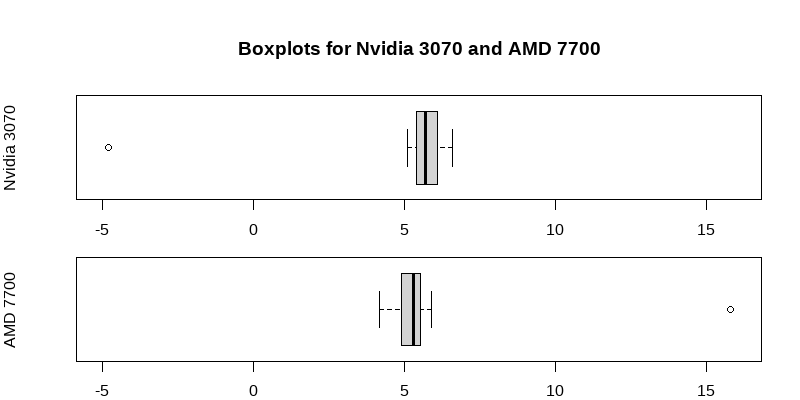
\includegraphics[width=0.75\textwidth]{assets/box_plot}
    \caption{Krabicový graf znázorňující rozložení nárůstu FPS po aplikaci 1.5 patche ve hře "Cyberpunk 2077" pro grafické karty \nvidiaCard\ a \amdCard}
    \label{fig:box_plot}
\end{figure}

\begin{figure}[h!]
    \centering
    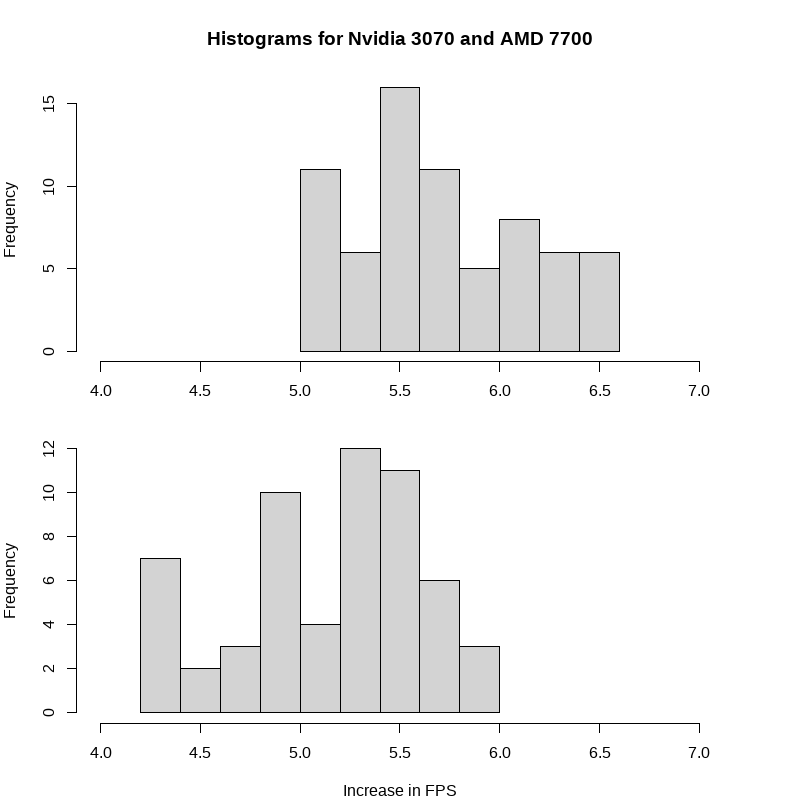
\includegraphics[width=0.75\textwidth]{assets/histogram}
    \caption{Histogram znázorňující rozložení nárůstu FPS po aplikaci 1.5 patche ve hře "Cyberpunk 2077" pro grafické karty \nvidiaCard\ a \amdCard}
    \label{fig:histogram}
\end{figure}

\begin{figure}[h!]
    \centering
    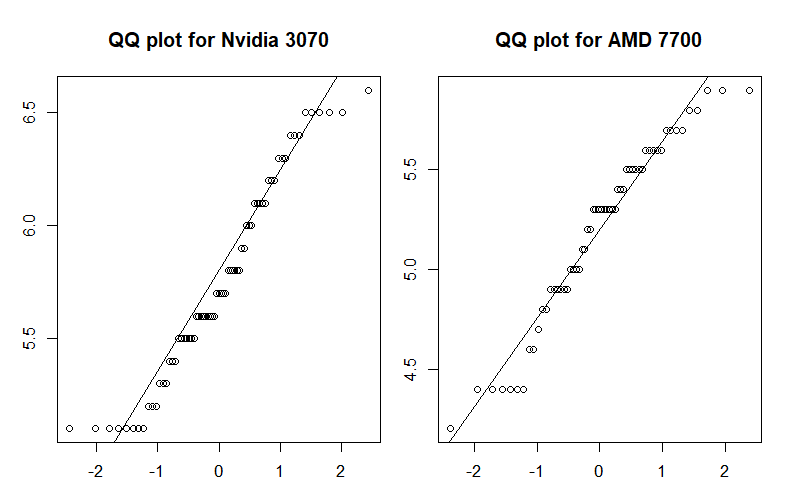
\includegraphics[width=0.85\textwidth]{assets/qq}
    \caption{Q-Q graf znázorňující nárůst FPS po aplikaci 1.5 patche ve hře "Cyberpunk 2077" pro grafické karty \nvidiaCard\ a \amdCard}
    \label{fig:qq}
\end{figure}

\newpage
\subsubsection*{Analýza nárůstu výkonnostních skóre (FPS) po aplikaci 1.5 patche ve hře "Cyberpunk 2077" pro grafickou kartu \nvidiaCard}

Během testu byl zjišťován nárůst FPS pro grafickou kartu \nvidiaCard\ ve hře "Cyberpunk 2077" mezi původním release a verzí s 1.5 patchem
pro \tableValue{\rangeValues}{0} testovacích systémů. Zjištěný nárůst FPS se pohyboval v rozmezí \tableValue{\minValues}{0} FPS
až \tableValue{\maxValues}{0} FPS. Nárůst FPS v testu č. 20 byl na základě metody vnitřních hradeb identifikován jako odlehlé pozorování
a nebude zahrnut do dalšího zpracování. Možné příčiny vzniku odlehlých pozorování jsou: Chyba při testování vzniklá náhlým výkyvem výkonu počítače
nebo chyba hardwaru výpočetní stanice. Dále uvedené výsledky tedy pocházejí z analýzy nárůstů FPS zjištěných u \tableValue{\rangeValues}{2}
testovacích systémů. Průměrný nárůst FPS byl \tableValue{\meanValues}{2} FPS, směrodatná odchylka pak \tableValue{\sdValues}{2} FPS\@.
U poloviny testovacích cyklů nárůst FPS nepřekročil \tableValue{\medianValues}{2} FPS. V polovině případů se nárůst FPS pohyboval v
rozmezí \tableValue{\QfValues}{2} FPS až \tableValue{\QtValues}{2} FPS. Vzhledem k povaze měřené veličiny není variační koeficient vhodnou mírou
pro posouzení variability souboru.

\vspace{1em}
\noindent
Výsledky pro grafickou kartu AMD Radeon RX 7700 XT lze komentovat obdobně.
Nárůst FPS se pohyboval v rozmezí \tableValue{\minValues}{1} až \tableValue{\maxValues}{1} FPS, s průměrným nárůstem \tableValue{\meanValues}{3} FPS a
směrodatnou odchylkou \tableValue{\sdValues}{3} FPS.\@
Za pomocí metody vnitřních hradeb bylo identifikováno odlehlé pozorování v testu č.\ 24, které bylo z analýzy vyloučeno.
Medián nárůstu činil \tableValue{\medianValues}{3} FPS, přičemž polovina výsledků spadala do intervalu \tableValue{\QfValues}{3} až \tableValue{\QtValues}{3} FPS.\@
Opět i zde není variační koeficient vhodným měřítkem variability souboru.

\subsubsection*{Ověření normality nárůstu výkonnostních skóre (FPS) po aplikaci 1.5 patche ve hře "Cyberpunk 2077" pro grafickou kartu \nvidiaCard}

Na základě grafického zobrazení (viz \figref{fig:qq}) u grafické karty \nvidiaCard\ a výběrové šikmosti a špičatosti (viz \tabref{tab:characteristics-summary},
výběrová šikmost a špičatost leží v intervalu (-2, 2)) lze předpokládat, že pozorovaný nárůst FPS má normální rozdělení. Dle pravidla 3$\sigma$ lze tedy očekávat,
že přibližně u 95 \% naměřených nárůstů ve výkonu bude \tableValue{\sigmaValues}{0} FPS až \tableValue{\sigmaValues}{1} FPS\@.

\subsubsection*{Ověření normality nárůstu výkonnostních skóre (FPS) po aplikaci 1.5 patche ve hře "Cyberpunk 2077" pro grafickou kartu \amdCard}

Na základě grafického zobrazení (viz \figref{fig:qq}) u grafické karty \amdCard\ a výběrové šikmosti a špičatosti (viz \tabref{tab:characteristics-summary},
výběrová šikmost a špičatost leží v intervalu (-2, 2)) lze předpokládat, že pozorovaný nárůst FPS má normální rozdělení. Dle pravidla 3$\sigma$ lze tedy očekávat,
že přibližně u 95 \% naměřených nárůstů ve výkonu bude \tableValue{\sigmaValues}{2} FPS až \tableValue{\sigmaValues}{3} FPS\@.

\endinput

%\newpage
%\section*{Úkol 2}
\label{sec:task-2}

Porovnejte nárůsty ve výkonnostních skórech (FPS) pro verzi hry "Cyberpunk 2077" po aplikaci 1.5 patche (dále jen \textbf{„nárůst FPS“}) 
pro vybrané grafické karty. Nezapomeňte, že použité metody mohou vyžadovat splnění určitých předpokladů. Pokud tomu tak bude, okomentujte 
splnění/nesplnění těchto předpokladů jak na základě explorační analýzy (např. s odkazem na histogram apod.), tak exaktně pomocí metod statistické indukce.

\begin{enumerate}[label=\alph*]
    \item Graficky prezentujte srovnání nárůstu FPS pro grafické karty Nvidia RTX 3070 Ti a AMD Radeon RX 7700 XT (vícenásobný krabicový graf, histogramy, q-q grafy). 
    Srovnání okomentujte (včetně informace o případné manipulaci s datovým souborem). 
    \textbf{Poznámka:} \textit{Byla-li grafická prezentace FPS v úkolu 1 bez připomínek, stačí do komentáře vložit odkaz na grafické výstupy z úkolu 1.}

    \newpage
    \item Na hladině významnosti 5 \% rozhodněte, zda jsou střední hodnoty nárůstů FPS (popř. mediány nárustů FPS) pro grafické karty Nvidia RTX 3070 Ti a 
    AMD Radeon RX 7700 XT statisticky významné. K řešení využijte bodové a intervalové odhady i čistý test významnosti. Výsledky okomentujte.

    \newpage
    \item Pro grafické karty Nvidia RTX 3070 Ti a AMD Radeon RX 7700 XT rozhodněte (na hladině významnosti 5 \%), zda se jejich střední hodnoty (popř. mediány) 
    nárůstu FPS po aplikaci 1.5 patche statisticky významně liší. K řešení využijte bodový a intervalový odhad i čistý test významnosti. Výsledky okomentujte.
\end{enumerate}

\endinput

%\newpage
%\section*{Úkol 3}
\label{sec:task-3}

Na hladině významnosti 5 \% rozhodněte, zda střední hodnoty (popř. mediány) nárůstů FPS po aplikaci 1.5 patche statisticky významně závisí na typu 
grafické karty. Posouzení proveďte nejprve na základě explorační analýzy a následně pomocí vhodného statistického testu, včetně ověření potřebných 
předpokladů. V případě, že se nárůst FPS pro různé grafické karty statisticky významně liší, určete pořadí karet dle středního nárůstu FPS (popř. mediánu nárůstu FPS). 
\textbf{Poznámka:} \textit{Srovnání proveďte pro všechny čtyři typy grafických karet.}

\begin{enumerate}[label=\alph*]
    \item Daný problém vhodným způsobem graficky prezentujte (vícenásobný krabicový graf, histogramy, q-q grafy). 
    Srovnání okomentujte (včetně informace o případné manipulaci s datovým souborem).
    
    \newpage
    \item Ověřte normalitu a symetrii nárůstů FPS u všech čtyř grafických karet (empiricky i exaktně).
    
    \newpage
    \item Ověřte homoskedasticitu (shodu rozptylů) nárůstů FPS mezi jednotlivými kartami (empiricky i exaktně)
    
    \newpage
    \item Určete bodové a 95\% intervalové odhady střední hodnoty (popř. mediánu) nárůstů FPS pro všechny srovnávané karty. 
    Volbu charakteristik proveďte tak, aby byly v souladu se statistickým testem, který plánujete provést v bodě e). 
    (Nezapomeňte na ověření předpokladů pro použití příslušných intervalových odhadů.)
    
    \newpage
    \item Čistým testem významnosti ověřte, zda je pozorovaný rozdíl středních hodnot (popř. mediánů) nárůstů FPS statisticky 
    významný na hladině významnosti 5\%. Pokud ano, zjistěte, zda lze některé skupiny karet označit (z hlediska nárůstů FPS)
    za homogenní, tj. určete pořadí karet dle středních hodnot (popř. mediánů) nárůstů FPS. 
    (Nezapomeňte na ověření předpokladů pro použití zvoleného testu.)
\end{enumerate}

\endinput

%\newpage
%\subsection*{Jak identifikovat, zda jsou v datech odlehlá pozorování?}
\label{subsec:how-to-identify-outliers}

\noindent
\textul{Empirické posouzení:}
\begin{itemize}
    \item použití vnitřních (vnějších) hradeb
    \item vizuální posouzení krabicového grafu.
\end{itemize}

\noindent 
Jak naložit s odlehlými hodnotami by měl definovat hlavně zadavatel analýzy (expert na danou problematiku).

\subsection*{Jak ověřit normalitu dat?}
\label{subsec:how-to-verify-normality}

\noindent
\textul{Empirické posouzení:}
\begin{itemize}
    \item vizuální posouzení histogramu,
    \item vizuální posouzení grafu odhadu hustoty pravděpodobnosti,
    \item Q-Q graf,
    \item posouzení výběrové šikmosti a výběrové špičatosti.
\end{itemize}

\noindent
\textul{Exaktní posouzení:}
\begin{itemize}
    \item testy normality (např. Shapirův – Wilkův test, Andersonův-Darlingův test, Lillieforsův test, ...)
\end{itemize}

\subsection*{Jak ověřit homoskedasticitu (shodu rozptylů)?}
\label{subsec:how-to-verify-homoscedasticity}

\noindent
\textul{Empirické posouzení:}
\begin{itemize}
    \item poměr největšího a nejmenšího rozptylu,
    \item vizuální posouzení krabicového grafu.
\end{itemize}

\noindent
\textul{Exaktní posouzení:}
\begin{itemize}
    \item F – test (parametrický dvouvýběrový test),
    \item Bartlettův test (parametrický vícevýběrový test),
    \item Leveneův test (neparametrický test).
\end{itemize}

\endinput

\end{document}